% Eigenvalue DOF-sweep spectra, colour variant (method by colour, DOF level by
% line style; index n vs eigenvalue lambda_n, several DOFs per method, against
% the analytic ground truth where available).
%
% Requires in the preamble:
%   \usepackage{graphicx}
%   \usepackage{subfig}
%
% The figures live next to this file, in results-paper/eigenvalues_dof_sweep/.
% If you \input this snippet from elsewhere, point graphicx at that folder, e.g.
%   \graphicspath{{results-paper/eigenvalues_dof_sweep/}}
% and drop the leading path from the \includegraphics arguments below.

\begin{figure}[htbp]
  \centering
  \subfloat[Rectangle, length $2\pi$, height $\pi$.]{%
    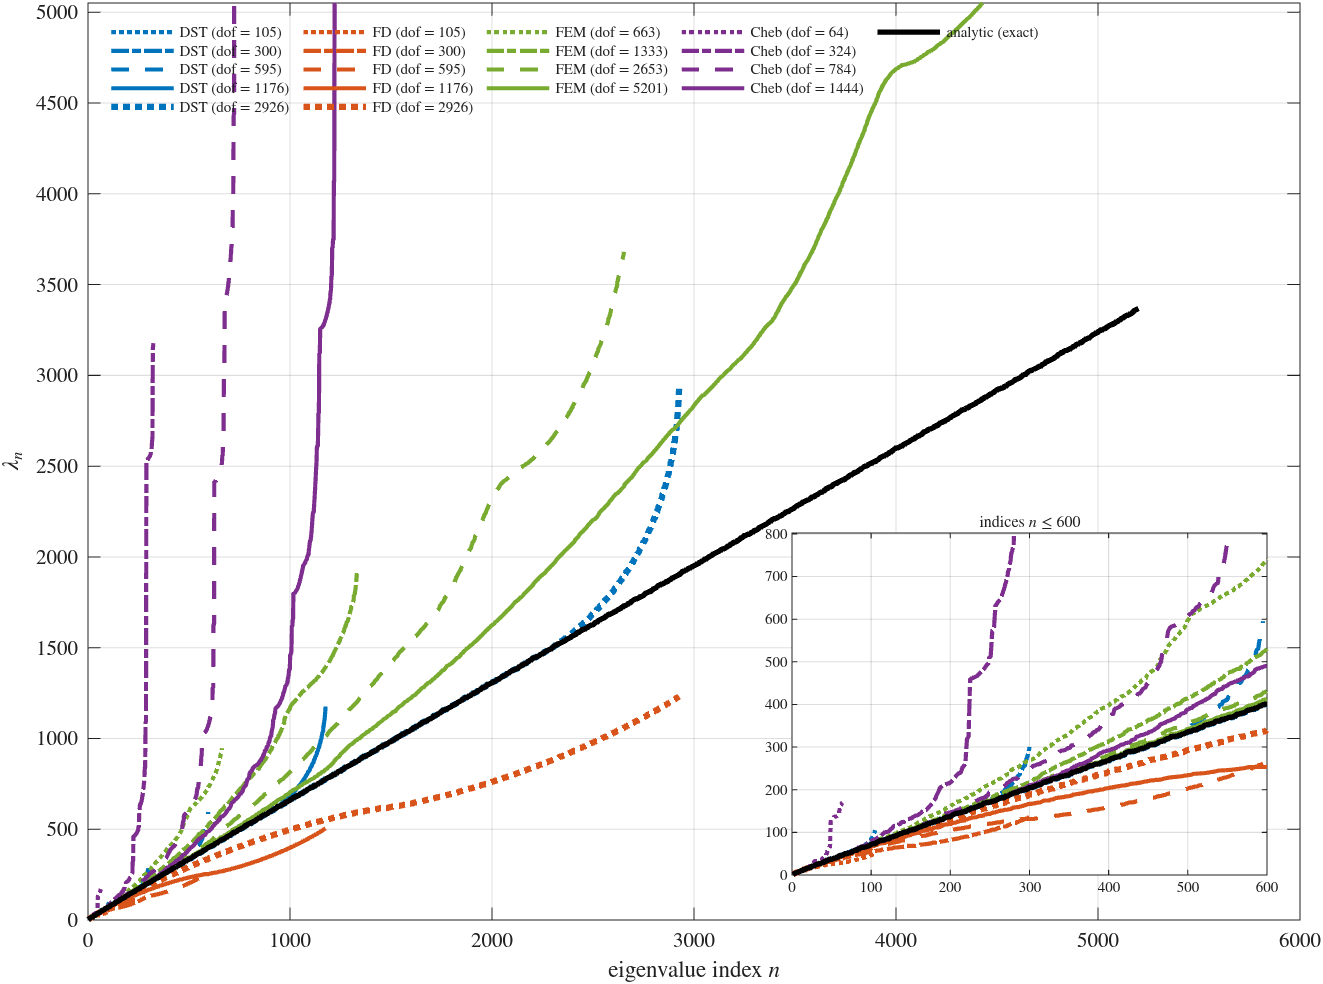
\includegraphics[width=0.8\textwidth]{rectangle_dof_sweep_colour}}
  \\
  \subfloat[Right isosceles triangle, legs length~$\pi$.]{%
    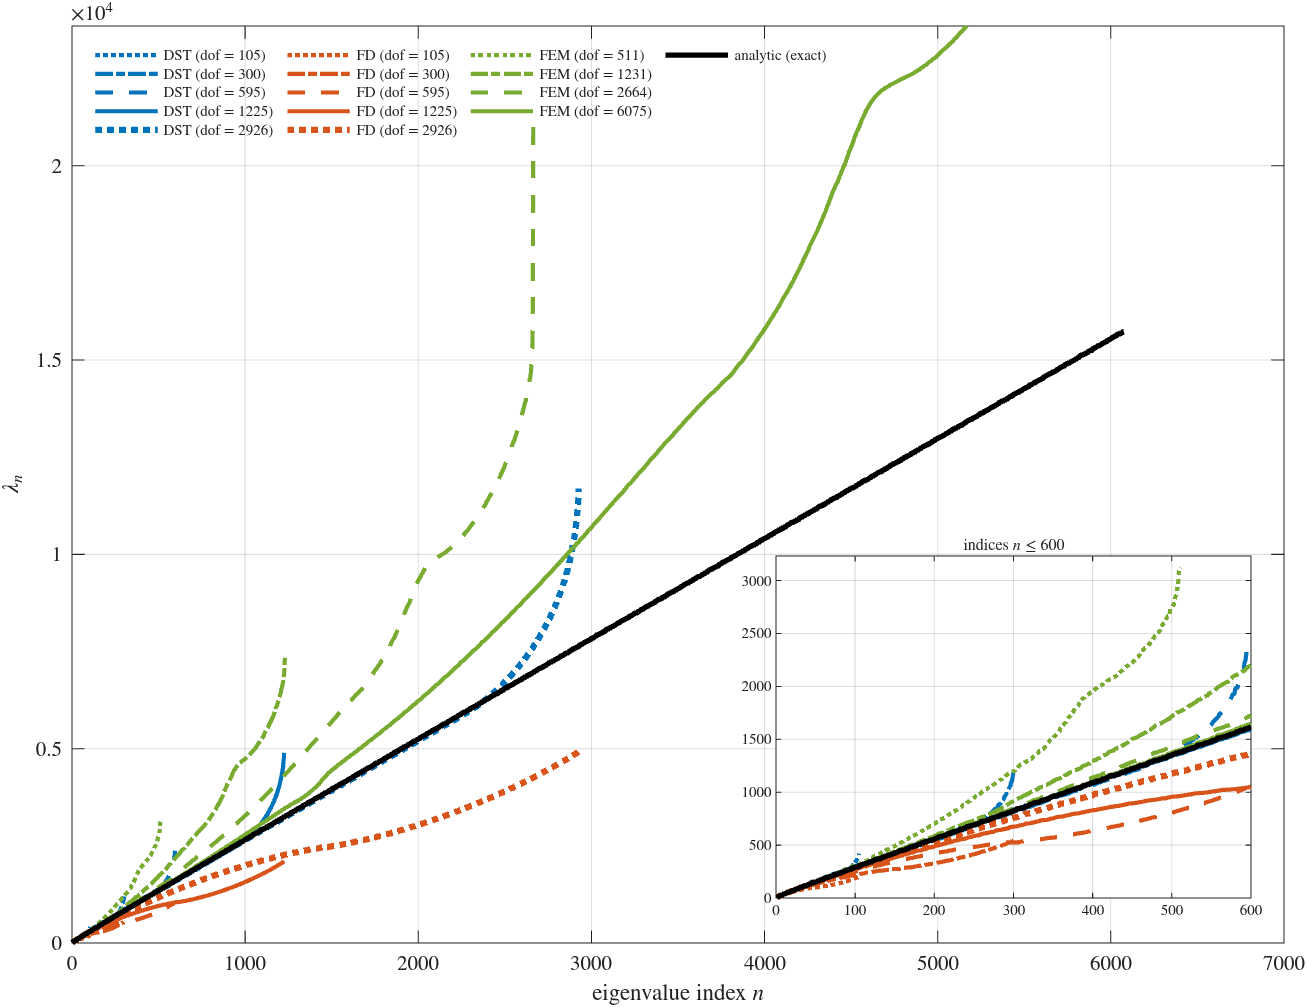
\includegraphics[width=0.8\textwidth]{isosceles_triangle_dof_sweep_colour}}
  \caption{Computed eigenvalues for various discretisations and their comparison with analytical eigenvalues of the Laplace operator with zero Dirichlet boundary conditions; rectangle and isosceles triangle. \texttt{FEM} -- finite element method, \texttt{FD} -- finite differences method, \texttt{Cheb} -- Chebyshev spectral collocation method, \texttt{DST} -- discrete sine transform method.}
  \label{fig:dof_sweep_colour}
\end{figure}

\begin{figure}[htbp]
  \centering
  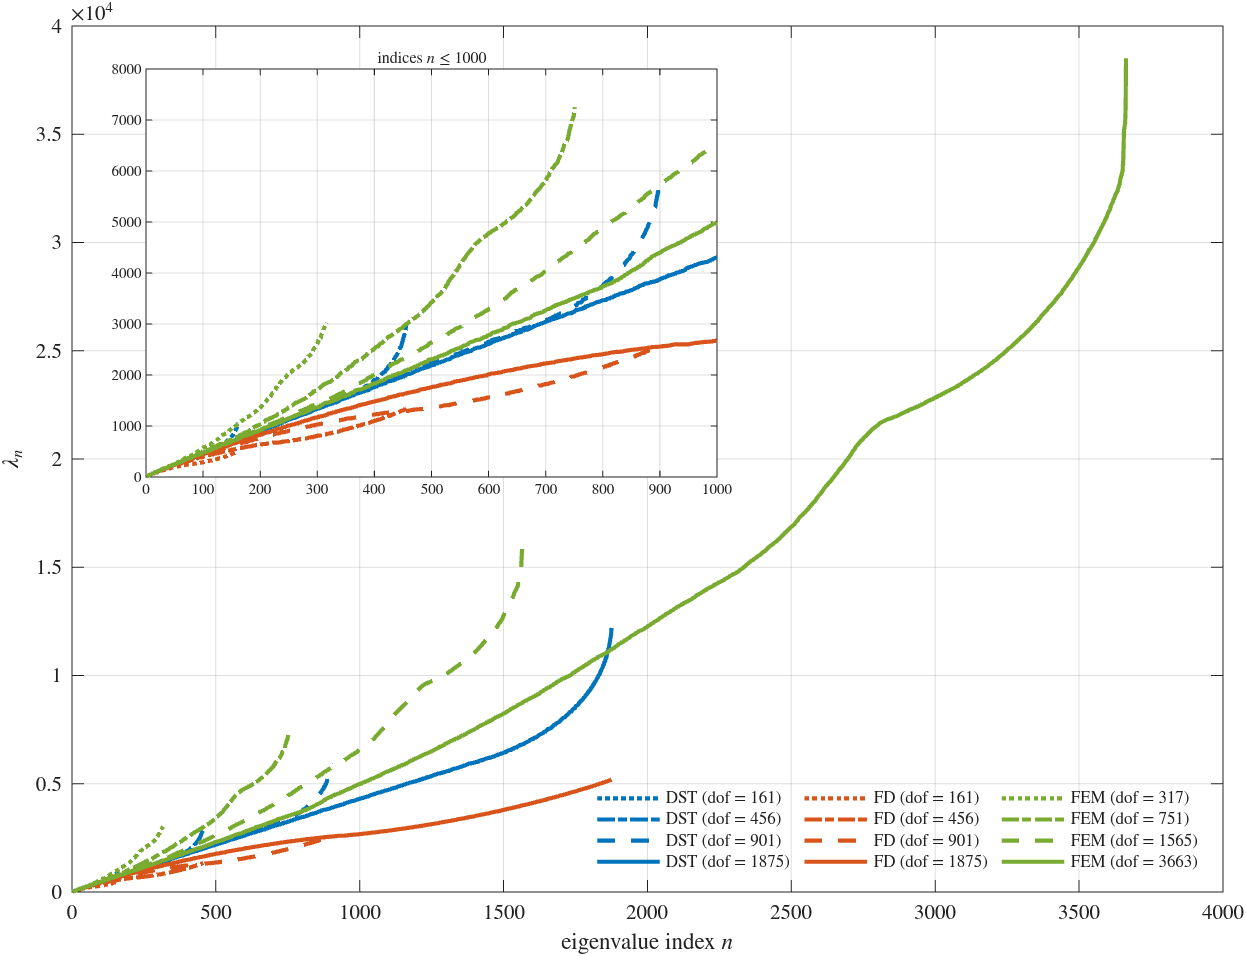
\includegraphics[width=0.8\textwidth]{L_shaped_dof_sweep_colour}
  \caption{Computed eigenvalues for various discretisations; L-shaped domain -- square domain $2 \times 2$ minus a $1 \times 1$ top right corner. \texttt{FEM} -- finite element method, \texttt{FD} -- finite differences method, \texttt{DST} -- discrete sine transform method.}
  \label{fig:dof_sweep_colour_L_shaped}
\end{figure}
